\documentclass[twoside]{book}

% Packages required by doxygen
\usepackage{fixltx2e}
\usepackage{calc}
\usepackage{doxygen}
\usepackage[export]{adjustbox} % also loads graphicx
\usepackage{graphicx}
\usepackage[utf8]{inputenc}
\usepackage{makeidx}
\usepackage{multicol}
\usepackage{multirow}
\PassOptionsToPackage{warn}{textcomp}
\usepackage{textcomp}
\usepackage[nointegrals]{wasysym}
\usepackage[table]{xcolor}

% Font selection
\usepackage[T1]{fontenc}
\usepackage[scaled=.90]{helvet}
\usepackage{courier}
\usepackage{amssymb}
\usepackage{sectsty}
\renewcommand{\familydefault}{\sfdefault}
\allsectionsfont{%
  \fontseries{bc}\selectfont%
  \color{darkgray}%
}
\renewcommand{\DoxyLabelFont}{%
  \fontseries{bc}\selectfont%
  \color{darkgray}%
}
\newcommand{\+}{\discretionary{\mbox{\scriptsize$\hookleftarrow$}}{}{}}

% Page & text layout
\usepackage{geometry}
\geometry{%
  a4paper,%
  top=2.5cm,%
  bottom=2.5cm,%
  left=2.5cm,%
  right=2.5cm%
}
\tolerance=750
\hfuzz=15pt
\hbadness=750
\setlength{\emergencystretch}{15pt}
\setlength{\parindent}{0cm}
\setlength{\parskip}{3ex plus 2ex minus 2ex}
\makeatletter
\renewcommand{\paragraph}{%
  \@startsection{paragraph}{4}{0ex}{-1.0ex}{1.0ex}{%
    \normalfont\normalsize\bfseries\SS@parafont%
  }%
}
\renewcommand{\subparagraph}{%
  \@startsection{subparagraph}{5}{0ex}{-1.0ex}{1.0ex}{%
    \normalfont\normalsize\bfseries\SS@subparafont%
  }%
}
\makeatother

% Headers & footers
\usepackage{fancyhdr}
\pagestyle{fancyplain}
\fancyhead[LE]{\fancyplain{}{\bfseries\thepage}}
\fancyhead[CE]{\fancyplain{}{}}
\fancyhead[RE]{\fancyplain{}{\bfseries\leftmark}}
\fancyhead[LO]{\fancyplain{}{\bfseries\rightmark}}
\fancyhead[CO]{\fancyplain{}{}}
\fancyhead[RO]{\fancyplain{}{\bfseries\thepage}}
\fancyfoot[LE]{\fancyplain{}{}}
\fancyfoot[CE]{\fancyplain{}{}}
\fancyfoot[RE]{\fancyplain{}{\bfseries\scriptsize Generated by Doxygen }}
\fancyfoot[LO]{\fancyplain{}{\bfseries\scriptsize Generated by Doxygen }}
\fancyfoot[CO]{\fancyplain{}{}}
\fancyfoot[RO]{\fancyplain{}{}}
\renewcommand{\footrulewidth}{0.4pt}
\renewcommand{\chaptermark}[1]{%
  \markboth{#1}{}%
}
\renewcommand{\sectionmark}[1]{%
  \markright{\thesection\ #1}%
}

% Indices & bibliography
\usepackage{natbib}
\usepackage[titles]{tocloft}
\setcounter{tocdepth}{3}
\setcounter{secnumdepth}{5}
\makeindex

% Hyperlinks (required, but should be loaded last)
\usepackage{ifpdf}
\ifpdf
  \usepackage[pdftex,pagebackref=true]{hyperref}
\else
  \usepackage[ps2pdf,pagebackref=true]{hyperref}
\fi
\hypersetup{%
  colorlinks=true,%
  linkcolor=blue,%
  citecolor=blue,%
  unicode%
}

% Custom commands
\newcommand{\clearemptydoublepage}{%
  \newpage{\pagestyle{empty}\cleardoublepage}%
}

\usepackage{caption}
\captionsetup{labelsep=space,justification=centering,font={bf},singlelinecheck=off,skip=4pt,position=top}

%===== C O N T E N T S =====

\begin{document}

% Titlepage & ToC
\hypersetup{pageanchor=false,
             bookmarksnumbered=true,
             pdfencoding=unicode
            }
\pagenumbering{alph}
\begin{titlepage}
\vspace*{7cm}
\begin{center}%
{\Large My Project }\\
\vspace*{1cm}
{\large Generated by Doxygen 1.8.13}\\
\end{center}
\end{titlepage}
\clearemptydoublepage
\pagenumbering{roman}
\tableofcontents
\clearemptydoublepage
\pagenumbering{arabic}
\hypersetup{pageanchor=true}

%--- Begin generated contents ---
\chapter{Hierarchical Index}
\section{Class Hierarchy}
This inheritance list is sorted roughly, but not completely, alphabetically\+:\begin{DoxyCompactList}
\item \contentsline{section}{Converter\+Options}{\pageref{class_converter_options}}{}
\item \contentsline{section}{Db\+Manager}{\pageref{class_db_manager}}{}
\item Q\+List\+Widget\begin{DoxyCompactList}
\item \contentsline{section}{Db\+Names\+List\+View}{\pageref{class_db_names_list_view}}{}
\end{DoxyCompactList}
\item Q\+Main\+Window\begin{DoxyCompactList}
\item \contentsline{section}{Main\+Window}{\pageref{class_main_window}}{}
\end{DoxyCompactList}
\item Q\+Object\begin{DoxyCompactList}
\item \contentsline{section}{C\+S\+V\+Table}{\pageref{class_c_s_v_table}}{}
\end{DoxyCompactList}
\item Q\+Tab\+Widget\begin{DoxyCompactList}
\item \contentsline{section}{Db\+Tables\+View}{\pageref{class_db_tables_view}}{}
\end{DoxyCompactList}
\item \contentsline{section}{Sql\+Model\+Converter}{\pageref{class_sql_model_converter}}{}
\end{DoxyCompactList}

\chapter{Class Index}
\section{Class List}
Here are the classes, structs, unions and interfaces with brief descriptions\+:\begin{DoxyCompactList}
\item\contentsline{section}{\hyperlink{class_abstract_db_model}{Abstract\+Db\+Model} \\*Интерфейс для модели базы данных }{\pageref{class_abstract_db_model}}{}
\item\contentsline{section}{\hyperlink{class_button_group}{Button\+Group} \\*Виджет для группировки кнопок }{\pageref{class_button_group}}{}
\item\contentsline{section}{\hyperlink{class_converter_options}{Converter\+Options} \\*Класс настроек конвертера \hyperlink{class_sql_model_converter}{Sql\+Model\+Converter} }{\pageref{class_converter_options}}{}
\item\contentsline{section}{\hyperlink{class_c_s_v_table}{C\+S\+V\+Table} }{\pageref{class_c_s_v_table}}{}
\item\contentsline{section}{\hyperlink{class_db_manager}{Db\+Manager} \\*Класс для работы с базой данных. Содержит минимальный набор функций для работы с бд }{\pageref{class_db_manager}}{}
\item\contentsline{section}{\hyperlink{class_db_model}{Db\+Model} \\*Модель базы данных }{\pageref{class_db_model}}{}
\item\contentsline{section}{\hyperlink{class_db_names_list_view}{Db\+Names\+List\+View} \\*Представление для списка имён таблиц бд с возможностью выбора }{\pageref{class_db_names_list_view}}{}
\item\contentsline{section}{\hyperlink{class_db_tables_view}{Db\+Tables\+View} \\*Представление для бд }{\pageref{class_db_tables_view}}{}
\item\contentsline{section}{\hyperlink{class_main_window}{Main\+Window} }{\pageref{class_main_window}}{}
\item\contentsline{section}{\hyperlink{class_sql_model_converter}{Sql\+Model\+Converter} \\*Класс конвертера }{\pageref{class_sql_model_converter}}{}
\item\contentsline{section}{\hyperlink{class_toggle_button}{Toggle\+Button} \\*Кнопка-\/переключатель }{\pageref{class_toggle_button}}{}
\end{DoxyCompactList}

\chapter{Class Documentation}
\hypertarget{class_converter_options}{}\section{Converter\+Options Class Reference}
\label{class_converter_options}\index{Converter\+Options@{Converter\+Options}}


Класс настроек конвертера \mbox{\hyperlink{class_sql_model_converter}{Sql\+Model\+Converter}}.  




{\ttfamily \#include $<$Sql\+Model\+Converter.\+h$>$}

\subsection*{Public Member Functions}
\begin{DoxyCompactItemize}
\item 
\mbox{\hyperlink{class_converter_options_a99308bb0a82b2f0436a7236ffe1248b0}{Converter\+Options}} (Q\+String path=\char`\"{}\char`\"{}, Q\+String delim=\char`\"{}\char`\"{}, Q\+String eol=\char`\"{}\char`\"{})
\begin{DoxyCompactList}\small\item\em Конструктор настроек \end{DoxyCompactList}\item 
Q\+String \mbox{\hyperlink{class_converter_options_a8707c21da7c05009d27812ebe3b14c05}{get\+Path}} ()
\begin{DoxyCompactList}\small\item\em Геттер для path. \end{DoxyCompactList}\item 
Q\+String \mbox{\hyperlink{class_converter_options_ae2e25968130d28b79bc5bd1ae399a343}{get\+Delim}} ()
\begin{DoxyCompactList}\small\item\em Геттер для delim. \end{DoxyCompactList}\item 
Q\+String \mbox{\hyperlink{class_converter_options_aceb1c916ae42c07a21962b8bd0796540}{get\+End\+Of\+Line}} ()
\begin{DoxyCompactList}\small\item\em Геттер для eol. \end{DoxyCompactList}\item 
void \mbox{\hyperlink{class_converter_options_ad00e2c89e88aad4e4396ec2bc662c2c8}{set\+Path}} (Q\+String path)
\begin{DoxyCompactList}\small\item\em Сеттер для path. \end{DoxyCompactList}\item 
void \mbox{\hyperlink{class_converter_options_a5fa443d5b4b85ae865df5e7e242427d9}{set\+Delim}} (Q\+String delim)
\begin{DoxyCompactList}\small\item\em Сеттер для delim. \end{DoxyCompactList}\item 
void \mbox{\hyperlink{class_converter_options_ad536240705b539c58323240ca5bc1f5c}{set\+End\+Of\+Line}} (Q\+String eol)
\begin{DoxyCompactList}\small\item\em Сеттер для eol. \end{DoxyCompactList}\end{DoxyCompactItemize}
\subsection*{Friends}
\begin{DoxyCompactItemize}
\item 
\mbox{\Hypertarget{class_converter_options_ac2834b7186dba9c25da67cb842f271f1}\label{class_converter_options_ac2834b7186dba9c25da67cb842f271f1}} 
class {\bfseries Sql\+Model\+Converter}
\end{DoxyCompactItemize}


\subsection{Detailed Description}
Класс настроек конвертера \mbox{\hyperlink{class_sql_model_converter}{Sql\+Model\+Converter}}. 

\subsection{Constructor \& Destructor Documentation}
\mbox{\Hypertarget{class_converter_options_a99308bb0a82b2f0436a7236ffe1248b0}\label{class_converter_options_a99308bb0a82b2f0436a7236ffe1248b0}} 
\index{Converter\+Options@{Converter\+Options}!Converter\+Options@{Converter\+Options}}
\index{Converter\+Options@{Converter\+Options}!Converter\+Options@{Converter\+Options}}
\subsubsection{\texorpdfstring{Converter\+Options()}{ConverterOptions()}}
{\footnotesize\ttfamily Converter\+Options\+::\+Converter\+Options (\begin{DoxyParamCaption}\item[{Q\+String}]{path = {\ttfamily \char`\"{}\char`\"{}},  }\item[{Q\+String}]{delim = {\ttfamily \char`\"{}\char`\"{}},  }\item[{Q\+String}]{eol = {\ttfamily \char`\"{}\char`\"{}} }\end{DoxyParamCaption})\hspace{0.3cm}{\ttfamily [inline]}}



Конструктор настроек 


\begin{DoxyParams}{Parameters}
{\em path} & Путь для сохранения csv-\/файлов, сформированных из бд \\
\hline
{\em delim} & Разделитель в csv-\/файле \\
\hline
{\em eol} & Символ конца строки в csv-\/файле \\
\hline
\end{DoxyParams}


\subsection{Member Function Documentation}
\mbox{\Hypertarget{class_converter_options_ae2e25968130d28b79bc5bd1ae399a343}\label{class_converter_options_ae2e25968130d28b79bc5bd1ae399a343}} 
\index{Converter\+Options@{Converter\+Options}!get\+Delim@{get\+Delim}}
\index{get\+Delim@{get\+Delim}!Converter\+Options@{Converter\+Options}}
\subsubsection{\texorpdfstring{get\+Delim()}{getDelim()}}
{\footnotesize\ttfamily Q\+String Converter\+Options\+::get\+Delim (\begin{DoxyParamCaption}{ }\end{DoxyParamCaption})\hspace{0.3cm}{\ttfamily [inline]}}



Геттер для delim. 

\begin{DoxyReturn}{Returns}
Q\+String 
\end{DoxyReturn}
\mbox{\Hypertarget{class_converter_options_aceb1c916ae42c07a21962b8bd0796540}\label{class_converter_options_aceb1c916ae42c07a21962b8bd0796540}} 
\index{Converter\+Options@{Converter\+Options}!get\+End\+Of\+Line@{get\+End\+Of\+Line}}
\index{get\+End\+Of\+Line@{get\+End\+Of\+Line}!Converter\+Options@{Converter\+Options}}
\subsubsection{\texorpdfstring{get\+End\+Of\+Line()}{getEndOfLine()}}
{\footnotesize\ttfamily Q\+String Converter\+Options\+::get\+End\+Of\+Line (\begin{DoxyParamCaption}{ }\end{DoxyParamCaption})\hspace{0.3cm}{\ttfamily [inline]}}



Геттер для eol. 

\begin{DoxyReturn}{Returns}
Q\+String 
\end{DoxyReturn}
\mbox{\Hypertarget{class_converter_options_a8707c21da7c05009d27812ebe3b14c05}\label{class_converter_options_a8707c21da7c05009d27812ebe3b14c05}} 
\index{Converter\+Options@{Converter\+Options}!get\+Path@{get\+Path}}
\index{get\+Path@{get\+Path}!Converter\+Options@{Converter\+Options}}
\subsubsection{\texorpdfstring{get\+Path()}{getPath()}}
{\footnotesize\ttfamily Q\+String Converter\+Options\+::get\+Path (\begin{DoxyParamCaption}{ }\end{DoxyParamCaption})\hspace{0.3cm}{\ttfamily [inline]}}



Геттер для path. 

\begin{DoxyReturn}{Returns}
Q\+String 
\end{DoxyReturn}
\mbox{\Hypertarget{class_converter_options_a5fa443d5b4b85ae865df5e7e242427d9}\label{class_converter_options_a5fa443d5b4b85ae865df5e7e242427d9}} 
\index{Converter\+Options@{Converter\+Options}!set\+Delim@{set\+Delim}}
\index{set\+Delim@{set\+Delim}!Converter\+Options@{Converter\+Options}}
\subsubsection{\texorpdfstring{set\+Delim()}{setDelim()}}
{\footnotesize\ttfamily void Converter\+Options\+::set\+Delim (\begin{DoxyParamCaption}\item[{Q\+String}]{delim }\end{DoxyParamCaption})\hspace{0.3cm}{\ttfamily [inline]}}



Сеттер для delim. 


\begin{DoxyParams}{Parameters}
{\em delim} & \\
\hline
\end{DoxyParams}
\mbox{\Hypertarget{class_converter_options_ad536240705b539c58323240ca5bc1f5c}\label{class_converter_options_ad536240705b539c58323240ca5bc1f5c}} 
\index{Converter\+Options@{Converter\+Options}!set\+End\+Of\+Line@{set\+End\+Of\+Line}}
\index{set\+End\+Of\+Line@{set\+End\+Of\+Line}!Converter\+Options@{Converter\+Options}}
\subsubsection{\texorpdfstring{set\+End\+Of\+Line()}{setEndOfLine()}}
{\footnotesize\ttfamily void Converter\+Options\+::set\+End\+Of\+Line (\begin{DoxyParamCaption}\item[{Q\+String}]{eol }\end{DoxyParamCaption})\hspace{0.3cm}{\ttfamily [inline]}}



Сеттер для eol. 


\begin{DoxyParams}{Parameters}
{\em eol} & \\
\hline
\end{DoxyParams}
\mbox{\Hypertarget{class_converter_options_ad00e2c89e88aad4e4396ec2bc662c2c8}\label{class_converter_options_ad00e2c89e88aad4e4396ec2bc662c2c8}} 
\index{Converter\+Options@{Converter\+Options}!set\+Path@{set\+Path}}
\index{set\+Path@{set\+Path}!Converter\+Options@{Converter\+Options}}
\subsubsection{\texorpdfstring{set\+Path()}{setPath()}}
{\footnotesize\ttfamily void Converter\+Options\+::set\+Path (\begin{DoxyParamCaption}\item[{Q\+String}]{path }\end{DoxyParamCaption})\hspace{0.3cm}{\ttfamily [inline]}}



Сеттер для path. 


\begin{DoxyParams}{Parameters}
{\em path} & \\
\hline
\end{DoxyParams}


The documentation for this class was generated from the following file\+:\begin{DoxyCompactItemize}
\item 
Sql\+Model\+Converter.\+h\end{DoxyCompactItemize}

\hypertarget{class_c_s_v_table}{}\section{C\+S\+V\+Table Class Reference}
\label{class_c_s_v_table}\index{C\+S\+V\+Table@{C\+S\+V\+Table}}
Inheritance diagram for C\+S\+V\+Table\+:\begin{figure}[H]
\begin{center}
\leavevmode
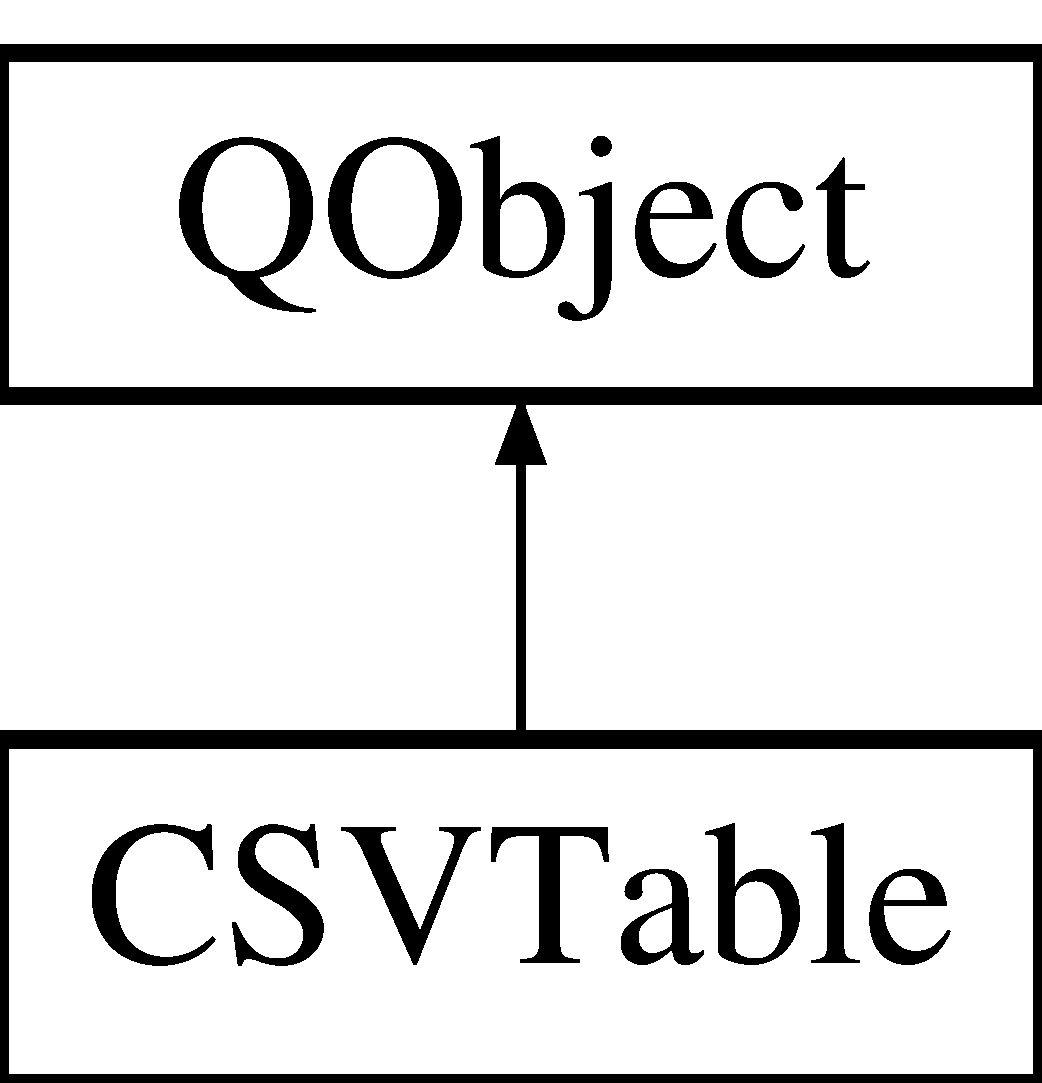
\includegraphics[height=2.000000cm]{class_c_s_v_table}
\end{center}
\end{figure}
\subsection*{Public Member Functions}
\begin{DoxyCompactItemize}
\item 
\mbox{\Hypertarget{class_c_s_v_table_aacf55dd84d5a852e2811e236dc6ab116}\label{class_c_s_v_table_aacf55dd84d5a852e2811e236dc6ab116}} 
{\bfseries C\+S\+V\+Table} (Q\+Object $\ast$parent)
\item 
\mbox{\Hypertarget{class_c_s_v_table_aa869da940a741a714a1de4c828f4a947}\label{class_c_s_v_table_aa869da940a741a714a1de4c828f4a947}} 
Error\+Code {\bfseries read} (const Q\+String \&filename, const Q\+String \&sep)
\end{DoxyCompactItemize}


The documentation for this class was generated from the following files\+:\begin{DoxyCompactItemize}
\item 
csvtable.\+h\item 
csvtable.\+cpp\end{DoxyCompactItemize}

\hypertarget{class_db_manager}{}\section{Db\+Manager Class Reference}
\label{class_db_manager}\index{Db\+Manager@{Db\+Manager}}


Класс для работы с базой данных. Содержит минимальный набор функций для работы с бд.  




{\ttfamily \#include $<$Db\+Manager.\+h$>$}

Inheritance diagram for Db\+Manager\+:\begin{figure}[H]
\begin{center}
\leavevmode
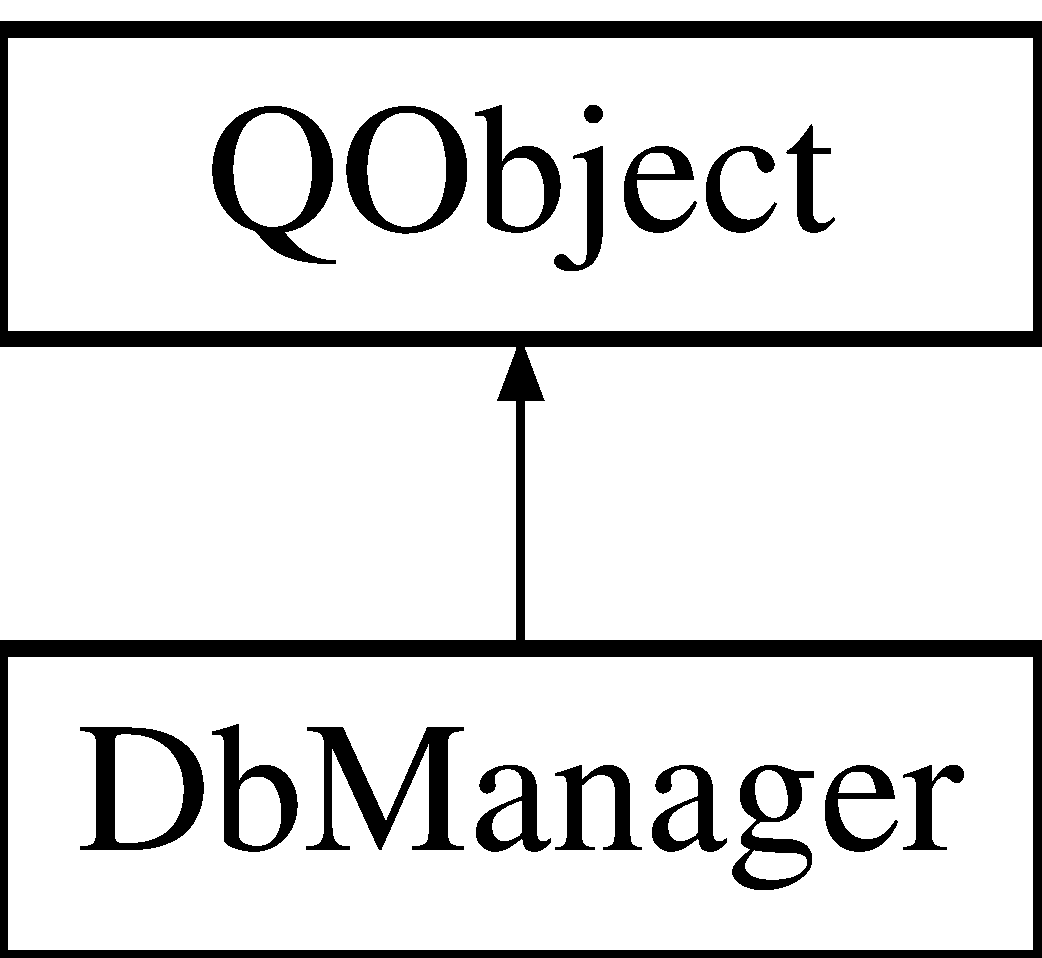
\includegraphics[height=2.000000cm]{class_db_manager}
\end{center}
\end{figure}
\subsection*{Public Member Functions}
\begin{DoxyCompactItemize}
\item 
\hyperlink{class_db_manager_acae386f0fc2af5d3f3b5c2adc5226391}{Db\+Manager} (const Q\+String \&path, Q\+String \&\&connection\+Name=\char`\"{}Default\char`\"{})
\item 
Q\+Sql\+Table\+Model $\ast$ \hyperlink{class_db_manager_a4b9a7828f0d6e53b695da5168570653c}{get\+Model} (const Q\+String \&table\+Name)
\begin{DoxyCompactList}\small\item\em Возвращает модель таблицы table\+Name, вызывая select() (см. Q\+Sql\+Table\+Model\+::select()) Удалять указатели не надо, они будут удалены при удалении менеджера бд \end{DoxyCompactList}\item 
Q\+String\+List \hyperlink{class_db_manager_a56efe9d49dc68dcdef05ae834f7618b0}{get\+Tables} ()
\begin{DoxyCompactList}\small\item\em Возвращает таблицы \end{DoxyCompactList}\item 
\mbox{\Hypertarget{class_db_manager_ac5cdf8e5e932d1681ab807d8f256374c}\label{class_db_manager_ac5cdf8e5e932d1681ab807d8f256374c}} 
\hyperlink{class_db_manager_ac5cdf8e5e932d1681ab807d8f256374c}{$\sim$\+Db\+Manager} ()
\begin{DoxyCompactList}\small\item\em Возвращает список с именами таблиц. \end{DoxyCompactList}\end{DoxyCompactItemize}
\subsection*{Public Attributes}
\begin{DoxyCompactItemize}
\item 
\mbox{\Hypertarget{class_db_manager_ad6b171f12dfc576b61c0c77bb7965285}\label{class_db_manager_ad6b171f12dfc576b61c0c77bb7965285}} 
Q\+Sql\+Database $\ast$ {\bfseries m\+\_\+db}
\end{DoxyCompactItemize}


\subsection{Detailed Description}
Класс для работы с базой данных. Содержит минимальный набор функций для работы с бд. 

\subsection{Constructor \& Destructor Documentation}
\mbox{\Hypertarget{class_db_manager_acae386f0fc2af5d3f3b5c2adc5226391}\label{class_db_manager_acae386f0fc2af5d3f3b5c2adc5226391}} 
\index{Db\+Manager@{Db\+Manager}!Db\+Manager@{Db\+Manager}}
\index{Db\+Manager@{Db\+Manager}!Db\+Manager@{Db\+Manager}}
\subsubsection{\texorpdfstring{Db\+Manager()}{DbManager()}}
{\footnotesize\ttfamily Db\+Manager\+::\+Db\+Manager (\begin{DoxyParamCaption}\item[{const Q\+String \&}]{path,  }\item[{Q\+String \&\&}]{connection\+Name = {\ttfamily \char`\"{}Default\char`\"{}} }\end{DoxyParamCaption})}


\begin{DoxyParams}[1]{Parameters}
\mbox{\tt in}  & {\em path} & Путь к базе данных\\
\hline
\mbox{\tt in}  & {\em connection\+Name} & Имя подключения к бд \\
\hline
\end{DoxyParams}


\subsection{Member Function Documentation}
\mbox{\Hypertarget{class_db_manager_a4b9a7828f0d6e53b695da5168570653c}\label{class_db_manager_a4b9a7828f0d6e53b695da5168570653c}} 
\index{Db\+Manager@{Db\+Manager}!get\+Model@{get\+Model}}
\index{get\+Model@{get\+Model}!Db\+Manager@{Db\+Manager}}
\subsubsection{\texorpdfstring{get\+Model()}{getModel()}}
{\footnotesize\ttfamily Q\+Sql\+Table\+Model $\ast$ Db\+Manager\+::get\+Model (\begin{DoxyParamCaption}\item[{const Q\+String \&}]{table\+Name }\end{DoxyParamCaption})}



Возвращает модель таблицы table\+Name, вызывая select() (см. Q\+Sql\+Table\+Model\+::select()) Удалять указатели не надо, они будут удалены при удалении менеджера бд 


\begin{DoxyParams}{Parameters}
{\em table\+Name\mbox{[}in\mbox{]}} & Имя таблицы, для которой надо вернуть модель \\
\hline
\end{DoxyParams}
\begin{DoxyReturn}{Returns}
Q\+Sql\+Table\+Model Модель для использования в представлении \hyperlink{class_db_tables_view}{Db\+Tables\+View} 
\end{DoxyReturn}
\mbox{\Hypertarget{class_db_manager_a56efe9d49dc68dcdef05ae834f7618b0}\label{class_db_manager_a56efe9d49dc68dcdef05ae834f7618b0}} 
\index{Db\+Manager@{Db\+Manager}!get\+Tables@{get\+Tables}}
\index{get\+Tables@{get\+Tables}!Db\+Manager@{Db\+Manager}}
\subsubsection{\texorpdfstring{get\+Tables()}{getTables()}}
{\footnotesize\ttfamily Q\+String\+List Db\+Manager\+::get\+Tables (\begin{DoxyParamCaption}{ }\end{DoxyParamCaption})}



Возвращает таблицы 

\begin{DoxyReturn}{Returns}
Q\+String\+List 
\end{DoxyReturn}


The documentation for this class was generated from the following files\+:\begin{DoxyCompactItemize}
\item 
Db\+Manager.\+h\item 
Db\+Manager.\+cpp\end{DoxyCompactItemize}

\hypertarget{class_db_names_list_view}{}\section{Db\+Names\+List\+View Class Reference}
\label{class_db_names_list_view}\index{Db\+Names\+List\+View@{Db\+Names\+List\+View}}


Представление для списка имён таблиц бд с возможностью выбора  




{\ttfamily \#include $<$Db\+Names\+List\+View.\+h$>$}

Inheritance diagram for Db\+Names\+List\+View\+:\begin{figure}[H]
\begin{center}
\leavevmode
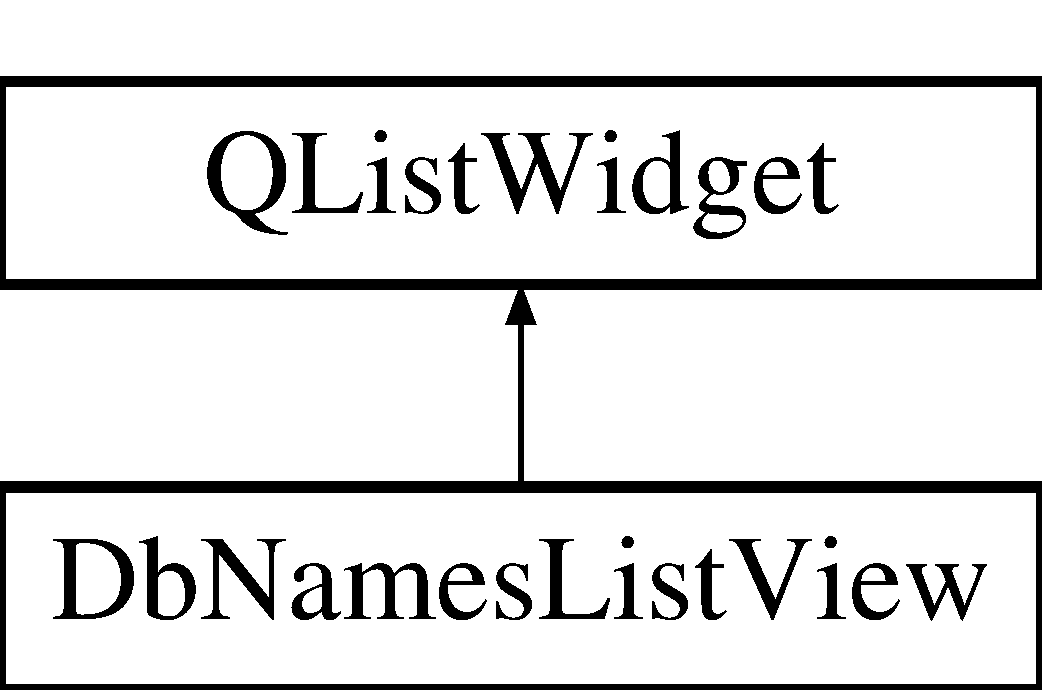
\includegraphics[height=2.000000cm]{class_db_names_list_view}
\end{center}
\end{figure}
\subsection*{Public Member Functions}
\begin{DoxyCompactItemize}
\item 
\hyperlink{class_db_names_list_view_a9898875686d3f621cf5e2be021e32b3c}{Db\+Names\+List\+View} (Q\+Widget $\ast$\&)
\begin{DoxyCompactList}\small\item\em Конструктор для преобразования(promotion) исходного класса qt. \end{DoxyCompactList}\item 
void \hyperlink{class_db_names_list_view_a323e31a217223ca8819030b455e88539}{Set\+Db\+Manager} (\hyperlink{class_db_manager}{Db\+Manager} $\ast$)
\begin{DoxyCompactList}\small\item\em Установить внутренний менеджер бд \end{DoxyCompactList}\item 
\mbox{\Hypertarget{class_db_names_list_view_a9c1889b82032cd1001b2fa1505eead11}\label{class_db_names_list_view_a9c1889b82032cd1001b2fa1505eead11}} 
void \hyperlink{class_db_names_list_view_a9c1889b82032cd1001b2fa1505eead11}{Fetch\+Tables} ()
\begin{DoxyCompactList}\small\item\em Загрузить информацию из бд в представление \end{DoxyCompactList}\item 
\mbox{\Hypertarget{class_db_names_list_view_a47edbf1349f633347f016d7496a55dab}\label{class_db_names_list_view_a47edbf1349f633347f016d7496a55dab}} 
void \hyperlink{class_db_names_list_view_a47edbf1349f633347f016d7496a55dab}{Clear} ()
\begin{DoxyCompactList}\small\item\em Очистить представление \end{DoxyCompactList}\item 
void \hyperlink{class_db_names_list_view_a14be2f72bf633024312843c43b353927}{Set\+And\+Fetch} (\hyperlink{class_db_manager}{Db\+Manager} $\ast$)
\begin{DoxyCompactList}\small\item\em Сокращение для Set\+Db\+Manager и Fetch\+Tables. \end{DoxyCompactList}\end{DoxyCompactItemize}


\subsection{Detailed Description}
Представление для списка имён таблиц бд с возможностью выбора 

\subsection{Constructor \& Destructor Documentation}
\mbox{\Hypertarget{class_db_names_list_view_a9898875686d3f621cf5e2be021e32b3c}\label{class_db_names_list_view_a9898875686d3f621cf5e2be021e32b3c}} 
\index{Db\+Names\+List\+View@{Db\+Names\+List\+View}!Db\+Names\+List\+View@{Db\+Names\+List\+View}}
\index{Db\+Names\+List\+View@{Db\+Names\+List\+View}!Db\+Names\+List\+View@{Db\+Names\+List\+View}}
\subsubsection{\texorpdfstring{Db\+Names\+List\+View()}{DbNamesListView()}}
{\footnotesize\ttfamily Db\+Names\+List\+View\+::\+Db\+Names\+List\+View (\begin{DoxyParamCaption}\item[{Q\+Widget $\ast$\&}]{p }\end{DoxyParamCaption})}



Конструктор для преобразования(promotion) исходного класса qt. 


\begin{DoxyParams}{Parameters}
{\em виджет-\/родитель} & \\
\hline
\end{DoxyParams}


\subsection{Member Function Documentation}
\mbox{\Hypertarget{class_db_names_list_view_a14be2f72bf633024312843c43b353927}\label{class_db_names_list_view_a14be2f72bf633024312843c43b353927}} 
\index{Db\+Names\+List\+View@{Db\+Names\+List\+View}!Set\+And\+Fetch@{Set\+And\+Fetch}}
\index{Set\+And\+Fetch@{Set\+And\+Fetch}!Db\+Names\+List\+View@{Db\+Names\+List\+View}}
\subsubsection{\texorpdfstring{Set\+And\+Fetch()}{SetAndFetch()}}
{\footnotesize\ttfamily void Db\+Names\+List\+View\+::\+Set\+And\+Fetch (\begin{DoxyParamCaption}\item[{\hyperlink{class_db_manager}{Db\+Manager} $\ast$}]{ }\end{DoxyParamCaption})}



Сокращение для Set\+Db\+Manager и Fetch\+Tables. 


\begin{DoxyParams}[1]{Parameters}
\mbox{\tt in}  & {\em Указатель} & на менеджер бд \\
\hline
\end{DoxyParams}
\mbox{\Hypertarget{class_db_names_list_view_a323e31a217223ca8819030b455e88539}\label{class_db_names_list_view_a323e31a217223ca8819030b455e88539}} 
\index{Db\+Names\+List\+View@{Db\+Names\+List\+View}!Set\+Db\+Manager@{Set\+Db\+Manager}}
\index{Set\+Db\+Manager@{Set\+Db\+Manager}!Db\+Names\+List\+View@{Db\+Names\+List\+View}}
\subsubsection{\texorpdfstring{Set\+Db\+Manager()}{SetDbManager()}}
{\footnotesize\ttfamily void Db\+Names\+List\+View\+::\+Set\+Db\+Manager (\begin{DoxyParamCaption}\item[{\hyperlink{class_db_manager}{Db\+Manager} $\ast$}]{db\+Manager }\end{DoxyParamCaption})}



Установить внутренний менеджер бд 


\begin{DoxyParams}[1]{Parameters}
\mbox{\tt in}  & {\em Указатель} & на менеджер бд \\
\hline
\end{DoxyParams}


The documentation for this class was generated from the following files\+:\begin{DoxyCompactItemize}
\item 
Db\+Names\+List\+View.\+h\item 
dbnameslistview.\+cpp\end{DoxyCompactItemize}

\hypertarget{class_db_tables_view}{}\section{Db\+Tables\+View Class Reference}
\label{class_db_tables_view}\index{Db\+Tables\+View@{Db\+Tables\+View}}


Представление для бд.  




{\ttfamily \#include $<$Db\+Tables\+View.\+h$>$}

Inheritance diagram for Db\+Tables\+View\+:\begin{figure}[H]
\begin{center}
\leavevmode
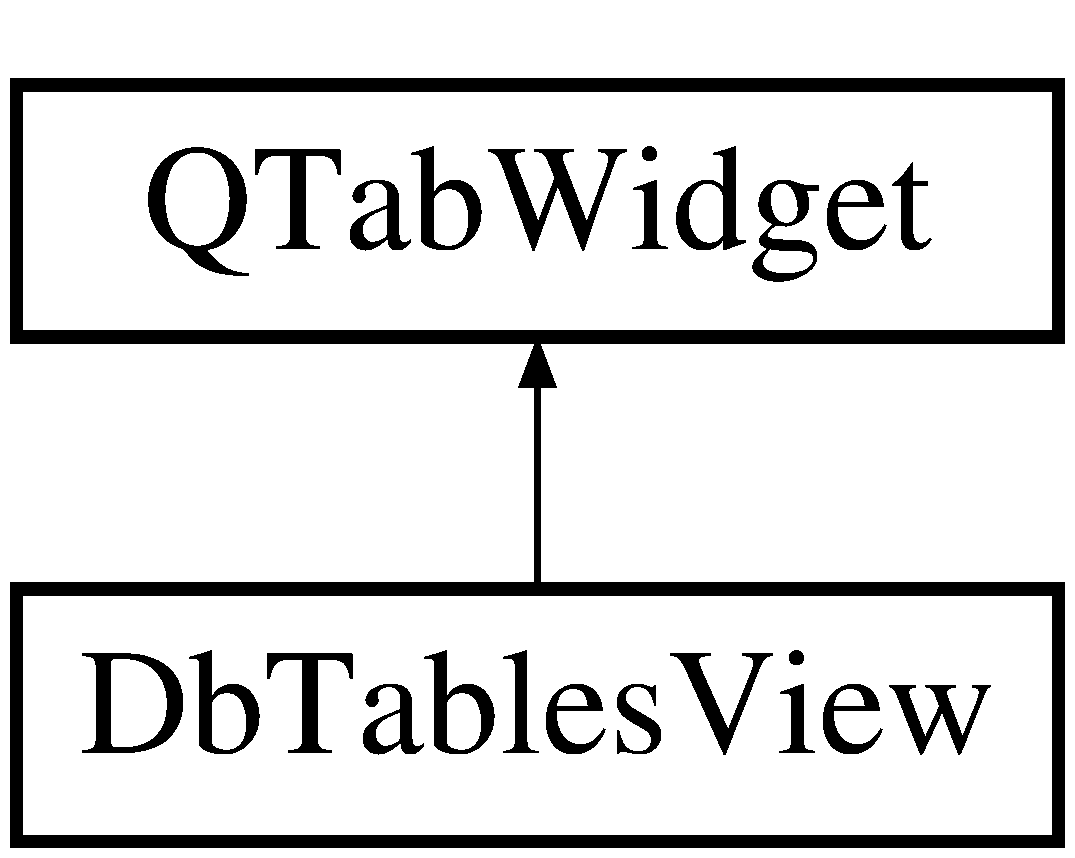
\includegraphics[height=2.000000cm]{class_db_tables_view}
\end{center}
\end{figure}
\subsection*{Public Member Functions}
\begin{DoxyCompactItemize}
\item 
\hyperlink{class_db_tables_view_a822d3b44cd293111709021a5f6d6799d}{Db\+Tables\+View} (Q\+Widget $\ast$\&)
\begin{DoxyCompactList}\small\item\em Конструктор для преобразования(promotion) исходного класса qt. \end{DoxyCompactList}\item 
void \hyperlink{class_db_tables_view_a0affcc4de194a59eff1ddbb68b88413e}{Set\+Db\+Manager} (\hyperlink{class_db_manager}{Db\+Manager} $\ast$)
\begin{DoxyCompactList}\small\item\em Устанавливает менеджер бд \end{DoxyCompactList}\item 
\mbox{\Hypertarget{class_db_tables_view_a85801e58584abc223bccc924ad707ead}\label{class_db_tables_view_a85801e58584abc223bccc924ad707ead}} 
void \hyperlink{class_db_tables_view_a85801e58584abc223bccc924ad707ead}{Fetch\+Tables} ()
\begin{DoxyCompactList}\small\item\em Загружает таблицы из предоставленного \hyperlink{class_db_manager}{Db\+Manager}. \end{DoxyCompactList}\item 
\mbox{\Hypertarget{class_db_tables_view_accf2ebff029e84812e48ca6564b392ef}\label{class_db_tables_view_accf2ebff029e84812e48ca6564b392ef}} 
void \hyperlink{class_db_tables_view_accf2ebff029e84812e48ca6564b392ef}{Clear} ()
\begin{DoxyCompactList}\small\item\em Очищает ресурсы, выделенные представлению \end{DoxyCompactList}\item 
void \hyperlink{class_db_tables_view_ad3d7529bd0acc4d08fe0d60616e96599}{Set\+And\+Fetch} (\hyperlink{class_db_manager}{Db\+Manager} $\ast$)
\begin{DoxyCompactList}\small\item\em Сокращение для Set\+Db\+Manager и Fetch\+Tables. \end{DoxyCompactList}\item 
Q\+Vector$<$ Q\+Sql\+Table\+Model $\ast$ $>$ \hyperlink{class_db_tables_view_adfe2d826189cb96dba5e8c4908911141}{get\+Models} ()
\begin{DoxyCompactList}\small\item\em Возвращает модели таблтц в бд \end{DoxyCompactList}\end{DoxyCompactItemize}


\subsection{Detailed Description}
Представление для бд. 

\subsection{Constructor \& Destructor Documentation}
\mbox{\Hypertarget{class_db_tables_view_a822d3b44cd293111709021a5f6d6799d}\label{class_db_tables_view_a822d3b44cd293111709021a5f6d6799d}} 
\index{Db\+Tables\+View@{Db\+Tables\+View}!Db\+Tables\+View@{Db\+Tables\+View}}
\index{Db\+Tables\+View@{Db\+Tables\+View}!Db\+Tables\+View@{Db\+Tables\+View}}
\subsubsection{\texorpdfstring{Db\+Tables\+View()}{DbTablesView()}}
{\footnotesize\ttfamily Db\+Tables\+View\+::\+Db\+Tables\+View (\begin{DoxyParamCaption}\item[{Q\+Widget $\ast$\&}]{p }\end{DoxyParamCaption})}



Конструктор для преобразования(promotion) исходного класса qt. 


\begin{DoxyParams}{Parameters}
{\em виджет-\/родитель} & \\
\hline
\end{DoxyParams}


\subsection{Member Function Documentation}
\mbox{\Hypertarget{class_db_tables_view_adfe2d826189cb96dba5e8c4908911141}\label{class_db_tables_view_adfe2d826189cb96dba5e8c4908911141}} 
\index{Db\+Tables\+View@{Db\+Tables\+View}!get\+Models@{get\+Models}}
\index{get\+Models@{get\+Models}!Db\+Tables\+View@{Db\+Tables\+View}}
\subsubsection{\texorpdfstring{get\+Models()}{getModels()}}
{\footnotesize\ttfamily Q\+Vector$<$ Q\+Sql\+Table\+Model $\ast$ $>$ Db\+Tables\+View\+::get\+Models (\begin{DoxyParamCaption}{ }\end{DoxyParamCaption})}



Возвращает модели таблтц в бд 

\begin{DoxyReturn}{Returns}
Q\+Vector$<$\+Q\+Sql\+Table\+Model $\ast$$>$ 
\end{DoxyReturn}
\mbox{\Hypertarget{class_db_tables_view_ad3d7529bd0acc4d08fe0d60616e96599}\label{class_db_tables_view_ad3d7529bd0acc4d08fe0d60616e96599}} 
\index{Db\+Tables\+View@{Db\+Tables\+View}!Set\+And\+Fetch@{Set\+And\+Fetch}}
\index{Set\+And\+Fetch@{Set\+And\+Fetch}!Db\+Tables\+View@{Db\+Tables\+View}}
\subsubsection{\texorpdfstring{Set\+And\+Fetch()}{SetAndFetch()}}
{\footnotesize\ttfamily void Db\+Tables\+View\+::\+Set\+And\+Fetch (\begin{DoxyParamCaption}\item[{\hyperlink{class_db_manager}{Db\+Manager} $\ast$}]{db\+Manager }\end{DoxyParamCaption})}



Сокращение для Set\+Db\+Manager и Fetch\+Tables. 


\begin{DoxyParams}[1]{Parameters}
\mbox{\tt in}  & {\em Указатель} & на менеджер бд \\
\hline
\end{DoxyParams}
\mbox{\Hypertarget{class_db_tables_view_a0affcc4de194a59eff1ddbb68b88413e}\label{class_db_tables_view_a0affcc4de194a59eff1ddbb68b88413e}} 
\index{Db\+Tables\+View@{Db\+Tables\+View}!Set\+Db\+Manager@{Set\+Db\+Manager}}
\index{Set\+Db\+Manager@{Set\+Db\+Manager}!Db\+Tables\+View@{Db\+Tables\+View}}
\subsubsection{\texorpdfstring{Set\+Db\+Manager()}{SetDbManager()}}
{\footnotesize\ttfamily void Db\+Tables\+View\+::\+Set\+Db\+Manager (\begin{DoxyParamCaption}\item[{\hyperlink{class_db_manager}{Db\+Manager} $\ast$}]{db\+Manager }\end{DoxyParamCaption})}



Устанавливает менеджер бд 


\begin{DoxyParams}[1]{Parameters}
\mbox{\tt in}  & {\em Указатель} & на менеджер бд \\
\hline
\end{DoxyParams}


The documentation for this class was generated from the following files\+:\begin{DoxyCompactItemize}
\item 
Db\+Tables\+View.\+h\item 
dbtablesview.\+cpp\end{DoxyCompactItemize}

\hypertarget{class_main_window}{}\section{Main\+Window Class Reference}
\label{class_main_window}\index{Main\+Window@{Main\+Window}}
Inheritance diagram for Main\+Window\+:\begin{figure}[H]
\begin{center}
\leavevmode
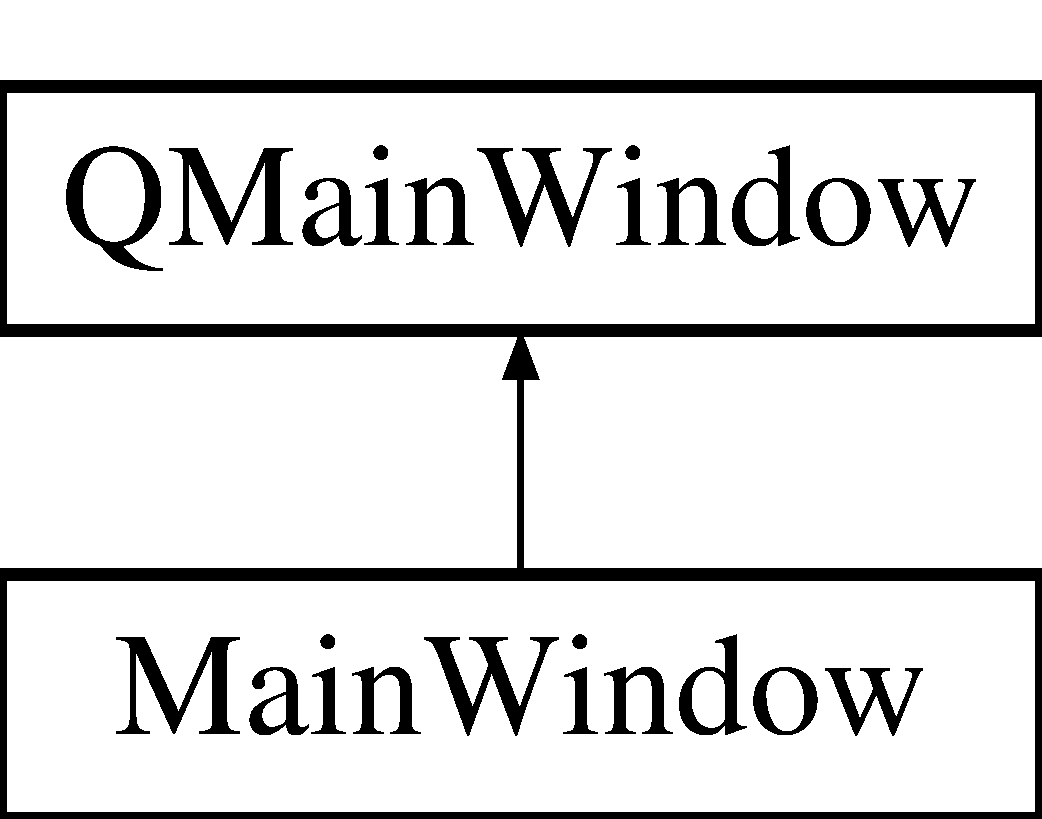
\includegraphics[height=2.000000cm]{class_main_window}
\end{center}
\end{figure}
\subsection*{Public Member Functions}
\begin{DoxyCompactItemize}
\item 
\mbox{\Hypertarget{class_main_window_a8b244be8b7b7db1b08de2a2acb9409db}\label{class_main_window_a8b244be8b7b7db1b08de2a2acb9409db}} 
{\bfseries Main\+Window} (Q\+Widget $\ast$parent=0)
\end{DoxyCompactItemize}
\subsection*{Public Attributes}
\begin{DoxyCompactItemize}
\item 
\mbox{\Hypertarget{class_main_window_a29a7d3c84689e952e3226a9d53d09cf4}\label{class_main_window_a29a7d3c84689e952e3226a9d53d09cf4}} 
\hyperlink{class_db_manager}{Db\+Manager} $\ast$ {\bfseries mngr} = nullptr
\item 
\mbox{\Hypertarget{class_main_window_a5556112edb83f621ccb8f53e067ec7a7}\label{class_main_window_a5556112edb83f621ccb8f53e067ec7a7}} 
Q\+Sql\+Table\+Model $\ast$ {\bfseries mdl} = nullptr
\end{DoxyCompactItemize}


The documentation for this class was generated from the following files\+:\begin{DoxyCompactItemize}
\item 
mainwindow.\+h\item 
mainwindow.\+cpp\end{DoxyCompactItemize}

\hypertarget{class_sql_model_converter}{}\section{Sql\+Model\+Converter Class Reference}
\label{class_sql_model_converter}\index{Sql\+Model\+Converter@{Sql\+Model\+Converter}}


Класс конвертера  




{\ttfamily \#include $<$Sql\+Model\+Converter.\+h$>$}

\subsection*{Public Member Functions}
\begin{DoxyCompactItemize}
\item 
\hyperlink{class_sql_model_converter_af7cf0d9772323b9707697f0ab4fc4e77}{Sql\+Model\+Converter} (Q\+String path=\char`\"{}\char`\"{}, Q\+String delim=\char`\"{},\char`\"{}, Q\+String end\+Of\+Line=\char`\"{}\textbackslash{})
\begin{DoxyCompactList}\small\item\em Конструктор конвертера Конструирует конвертер с заданными настройками \end{DoxyCompactList}\item 
\hyperlink{class_sql_model_converter_a9d2feafdb9c7568370f2c02bb7e5e64f}{Sql\+Model\+Converter} (\hyperlink{class_converter_options}{Converter\+Options})
\begin{DoxyCompactList}\small\item\em Конструктор конвертера Конструирует конвертер с заданными настройками \end{DoxyCompactList}\item 
void \hyperlink{class_sql_model_converter_a9cff9f1e0a7dfa36d0a34a8a3188f1ea}{sql\+To\+Csv} (const Q\+Vector$<$ Q\+Sql\+Table\+Model $\ast$$>$ \&models, const Q\+String\+List \&tables\+To\+Convert, Q\+Hash$<$ Q\+String, Q\+String $>$ \&result)
\begin{DoxyCompactList}\small\item\em Преобразует таблицы sql в csv-\/файлы Преобразует таблицы sql, заданные в форме моделей, в csv-\/файлы, согласно настройкам, установленным в конструкторе класса. \end{DoxyCompactList}\end{DoxyCompactItemize}
\subsection*{Public Attributes}
\begin{DoxyCompactItemize}
\item 
\hyperlink{class_converter_options}{Converter\+Options} \hyperlink{class_sql_model_converter_a562f55118cd1924c249796b6e183acbd}{options}
\end{DoxyCompactItemize}


\subsection{Detailed Description}
Класс конвертера 

\subsection{Constructor \& Destructor Documentation}
\mbox{\Hypertarget{class_sql_model_converter_af7cf0d9772323b9707697f0ab4fc4e77}\label{class_sql_model_converter_af7cf0d9772323b9707697f0ab4fc4e77}} 
\index{Sql\+Model\+Converter@{Sql\+Model\+Converter}!Sql\+Model\+Converter@{Sql\+Model\+Converter}}
\index{Sql\+Model\+Converter@{Sql\+Model\+Converter}!Sql\+Model\+Converter@{Sql\+Model\+Converter}}
\subsubsection{\texorpdfstring{Sql\+Model\+Converter()}{SqlModelConverter()}\hspace{0.1cm}{\footnotesize\ttfamily [1/2]}}
{\footnotesize\ttfamily Sql\+Model\+Converter\+::\+Sql\+Model\+Converter (\begin{DoxyParamCaption}\item[{Q\+String}]{path = {\ttfamily \char`\"{}\char`\"{}},  }\item[{Q\+String}]{delim = {\ttfamily \char`\"{},\char`\"{}},  }\item[{Q\+String}]{end\+Of\+Line = {\ttfamily \char`\"{}\textbackslash{}n\char`\"{}} }\end{DoxyParamCaption})}



Конструктор конвертера Конструирует конвертер с заданными настройками 


\begin{DoxyParams}{Parameters}
{\em path} & Путь для сохранения csv-\/файлов, сформированных из бд \\
\hline
{\em delim} & Разделитель в csv-\/файле \\
\hline
{\em end\+Of\+Line} & Символ конца строки в csv-\/файле \\
\hline
\end{DoxyParams}
\mbox{\Hypertarget{class_sql_model_converter_a9d2feafdb9c7568370f2c02bb7e5e64f}\label{class_sql_model_converter_a9d2feafdb9c7568370f2c02bb7e5e64f}} 
\index{Sql\+Model\+Converter@{Sql\+Model\+Converter}!Sql\+Model\+Converter@{Sql\+Model\+Converter}}
\index{Sql\+Model\+Converter@{Sql\+Model\+Converter}!Sql\+Model\+Converter@{Sql\+Model\+Converter}}
\subsubsection{\texorpdfstring{Sql\+Model\+Converter()}{SqlModelConverter()}\hspace{0.1cm}{\footnotesize\ttfamily [2/2]}}
{\footnotesize\ttfamily Sql\+Model\+Converter\+::\+Sql\+Model\+Converter (\begin{DoxyParamCaption}\item[{\hyperlink{class_converter_options}{Converter\+Options}}]{opts }\end{DoxyParamCaption})}



Конструктор конвертера Конструирует конвертер с заданными настройками 


\begin{DoxyParams}{Parameters}
{\em \hyperlink{class_converter_options}{Converter\+Options}} & Настройки конвертера \\
\hline
\end{DoxyParams}


\subsection{Member Function Documentation}
\mbox{\Hypertarget{class_sql_model_converter_a9cff9f1e0a7dfa36d0a34a8a3188f1ea}\label{class_sql_model_converter_a9cff9f1e0a7dfa36d0a34a8a3188f1ea}} 
\index{Sql\+Model\+Converter@{Sql\+Model\+Converter}!sql\+To\+Csv@{sql\+To\+Csv}}
\index{sql\+To\+Csv@{sql\+To\+Csv}!Sql\+Model\+Converter@{Sql\+Model\+Converter}}
\subsubsection{\texorpdfstring{sql\+To\+Csv()}{sqlToCsv()}}
{\footnotesize\ttfamily void Sql\+Model\+Converter\+::sql\+To\+Csv (\begin{DoxyParamCaption}\item[{const Q\+Vector$<$ Q\+Sql\+Table\+Model $\ast$$>$ \&}]{models,  }\item[{const Q\+String\+List \&}]{tables\+To\+Convert,  }\item[{Q\+Hash$<$ Q\+String, Q\+String $>$ \&}]{result }\end{DoxyParamCaption})}



Преобразует таблицы sql в csv-\/файлы Преобразует таблицы sql, заданные в форме моделей, в csv-\/файлы, согласно настройкам, установленным в конструкторе класса. 


\begin{DoxyParams}{Parameters}
{\em models} & Массив моделей таблиц \\
\hline
{\em tables\+To\+Convert} & Список имён таблиц, для которых надо выполнить преобразование \\
\hline
{\em result} & Словарь вида \char`\"{}Имя таблицы\char`\"{} -\/ \char`\"{}содержимое соответствующего csv-\/файла\char`\"{} \\
\hline
\end{DoxyParams}


\subsection{Member Data Documentation}
\mbox{\Hypertarget{class_sql_model_converter_a562f55118cd1924c249796b6e183acbd}\label{class_sql_model_converter_a562f55118cd1924c249796b6e183acbd}} 
\index{Sql\+Model\+Converter@{Sql\+Model\+Converter}!options@{options}}
\index{options@{options}!Sql\+Model\+Converter@{Sql\+Model\+Converter}}
\subsubsection{\texorpdfstring{options}{options}}
{\footnotesize\ttfamily \hyperlink{class_converter_options}{Converter\+Options} Sql\+Model\+Converter\+::options}

T\+O\+DO\+: describe 

The documentation for this class was generated from the following files\+:\begin{DoxyCompactItemize}
\item 
Sql\+Model\+Converter.\+h\item 
Sql\+Model\+Converter.\+cpp\end{DoxyCompactItemize}

%--- End generated contents ---

% Index
\backmatter
\newpage
\phantomsection
\clearemptydoublepage
\addcontentsline{toc}{chapter}{Index}
\printindex

\end{document}
